\selectlanguage{italian}
\section{Definizioni e nomenclatura}

Un nuclide (o nucleo) è una specifica combinazione di protoni e neutroni: si definiscono il numero atomico $ Z $ come il numero di protoni, il numero di neutroni $ N $ ed il numero di massa $ A = Z + N $ come il numero di nucleoni. In un atomo neutro, $ Z $ è anche il numero totale di elettroni negli orbitali.\\
Il simbolo completo di un nuclide è $ ^A_Z \text{X}_N $, dove $ \text{X} $ è il simbolo della specie chimica: tale scrittura è però ridondante, poiché la specie chimica definisce di per sé il numero di protoni nel nuclide, dunque è sufficiente scrivere $ ^A \text{X} $.\\
Nuclidi con lo stesso $ Z $ sono detti isotopi, con lo stesso $ A $ isobari e con lo stesso $ N $ isotoni.

\subsection{Unità di misura}

Nell'ambito della fisica nucleare e particellare è sconveniente utilizzare le unità di misura del Sistema Internazionale: unità di misura tipiche sono il fermi $ 1\fm = 10^{-15}\m $, l'elettronvolt $ 1\ev = 1.602\cdot10^{-19}\,\text{J} $ e l'unità di massa atomica $ 1\,\text{u} = 1.6606\cdot10^{-27}\,\text{kg} = 931.502 \mev/c^2 $ (definita come $ 1/12 $ della massa di un atomo di $ \ch{^{12}C} $).\\
Per semplificare le equazioni, è utile porre le costanti fondamentali $ c = \hbar = 1 $: questo sistema di misura è detto Sistema Naturale e in esso massa, momento lineare, energia, lunghezza$ ^{-1} $ e tempo$ ^{-1} $ hanno la stessa unità di misura, poiché le equazioni di Einstein, Plank e de Broglie diventano rispettivamente $ E^2 = m_0^2 + p^2 $, $ E = 2\pi \nu $ e $ \lambda = \frac{2\pi}{p} $.

\subsubsection{Masse e costanti}

Nel SI, è utile ricordare i seguenti valori approssimati delle costanti fondamentali:
\begin{equation*}
    \begin{split}
	  &c = 2.99792458\cdot10^8 \m/\text{s} \approx 3\cdot10^8 \m/\text{s}\\
	  &\hbar = 6.58211928\cdot10^{-22} \mev\,\text{s} \approx \frac{2}{3}\cdot10^{-21} \mev\,\text{s}\\
	  &\hbar c = 197.3269718 \mev\fm \approx 200 \mev\fm
    \end{split}
\end{equation*}

Si possono quindi esprimere le masse dei nucleoni e dell'elettrone in varie unità di misura:
\begin{equation*}
	\begin{split}
		&m_p = 1.673\cdot10^{-27}\,\text{kg} = 1.00728\,\text{u} = 938.279 \mev/c^2\\
		&m_n = 1.675\cdot10^{-27}\,\text{kg} = 1.00867\,\text{u} = 939.573 \mev/c^2\\
		&m_e = 9.110\cdot10^{-31}\,\text{kg} = 0.511\mev/c^2
	\end{split}
\end{equation*}

\subsection{La tavola di Segré}

Al pari delle specie chimiche nella tavola periodica, anche i nuclidi possono essere messi in una tabella, tipicamente in un piano $ Z - N $ (Fig. \ref{segre-chart}): questa viene detta tavola di Segré e permette di tracciare facilmente i vari decadimenti radioattivi dei nuclidi, visualizzando efficaciemente le decay chains.\\
Come si vede in Fig. \ref{drip-lines}, è possibile distinguere la tavola dei nuclidi in due regioni separate da due linee: queste sono dette nuclear driplines e distinguono tra configurazioni di protoni e neutroni che possono effettivamente formare dei nuclidi (sia stabili che instabili, ovvero radioattivi) e configurazioni nelle quali invece l'interazione forte non riesce a mantenere insieme i nucleoni per formare un nucleo. Si stima che possano esistere oltre $ 7000 $ nuclidi nell'Universo, ma di questi solo circa $ 3000 $ sono stati effettivamente scoperti (di cui solo $ 251 $ nuclidi stabili): si parla in questo caso di $ \virgolette{Terra incognita} $ per indicare il teoricamente alto numero di nuclidi ancora ignoti; in particolare, è stata teoricamente prevista un'$ \virgolette{isola} $ di elementi super-pesanti attorno a $ Z = 114 $ ed oltre, con nuclidi con vite medie dell'ordine di minuti o giorni: sebbene non ancora osservati, si pensa che la chimica degli elementi super-pesanti con $ Z > 118 $ sia di natura relativistica, dunque incomparabile a quella degli elementi fin'ora scoperti.

\begin{figure}
  \centering
  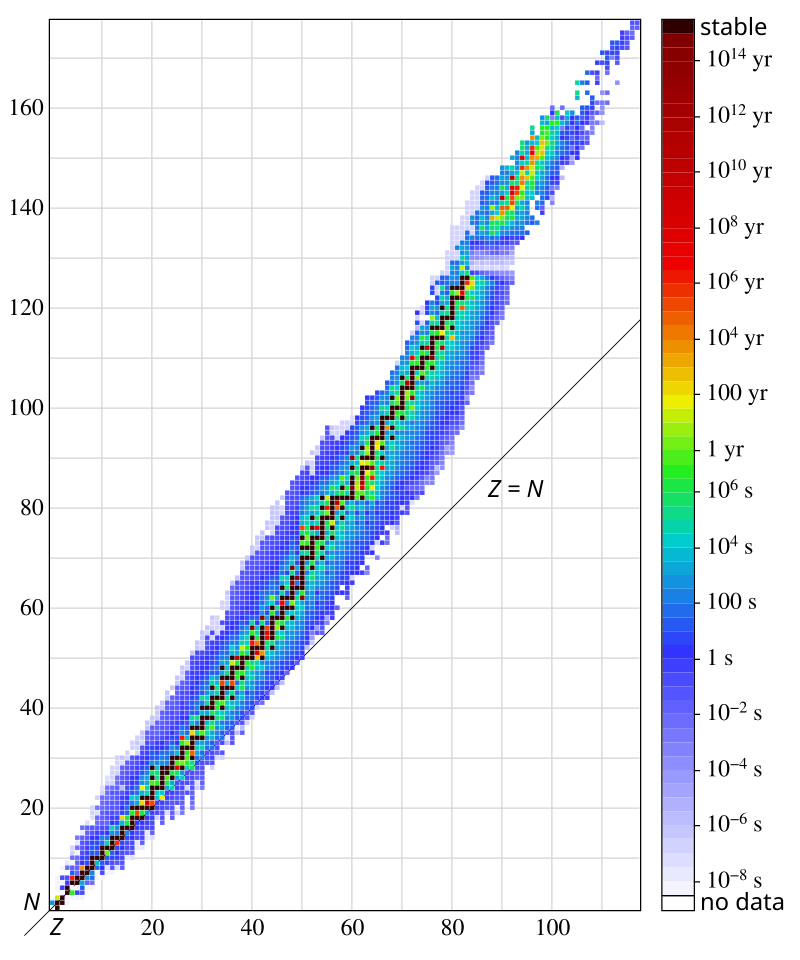
\includegraphics[width = 0.75\textwidth]{segre-chart.png}
  \caption{Tavola di Segré.}
  \label{segre-chart}
\end{figure}
\begin{figure}
  \centering
  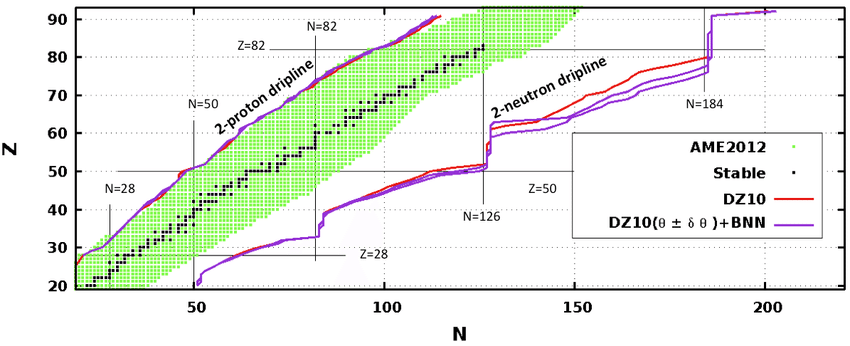
\includegraphics[width = 0.55\textwidth]{drip-lines.png}
  \caption{Nuclear driplines.}
  \label{drip-lines}
\end{figure}

\section{Evidenze sperimentali}

Le prime evidenze sperimentali dell'esistenza del nucleo atomico si devono al gruppo di ricerca di Rutherford, Geiger e Marsden: prima di loro, Thomson era riuscito ad estrarre delle cariche negative dall'atomo, identificando l'elettrone, ed aveva di conseguenza formulato la sua teoria della struttura atomica come sfera carica positivamente in cui sono immersi gli elettroni ($ \virgolette{plum pudding} $ model).\\
Con i loro esperimenti, Rutherford et al. dimostrarono invece che le cariche positive erano concentrate in una regione piccola al centro dell'atomo.

\subsection{Scattering di Rutherford}

L'esperimento condotto da Rutherford et al. consiste nell'irradiare una lamina sottile di oro con un fascio di particelle $ \alpha $ (nuclei di $ \ch{^{4} He} $): a livello puramente cinematico (ignorando la natura dell'interazione tra beam e target), essendo la velocità delle particelle $ \alpha $ $ v_0 \sim 0.1c $, è possibile trattare il problema come un urto elastico non-relativistico:
\begin{equation}
	\begin{cases}
	  m_{\alpha} \ve{v}_0 = m_{\alpha} \ve{v}_f + m_t \ve{v}_t \\
	  m_{\alpha} v_0^2 = m_{\alpha} v_f^2 + m_t v_t^2 \\
	\end{cases}
	\label{eq:2}
\end{equation}
Combinando le due equazioni e definendo $ \theta $ l'angolo tra $ \ve{v}_f $ e $ \ve{v}_t $:
\begin{equation}
	\cos \theta = \frac{1}{2} \frac{v_t}{v_f} \left(1 - \frac{m_t}{m_{\alpha}}\right)
	\label{eq:3}
\end{equation}
Si possono distinguere due principali casi:
\begin{enumerate}
	\item $ m_t \ll m_{\alpha} $: $ \cos \theta > 0 $, dunque si parla di forward scattering, poiché non sono possibili grossi valori di $ \theta $;
	\item $ m_t \gg m_{\alpha} $: $ \cos \theta < 0 $, dunque diventano possibili anche angoli prossimi $ \pi $.
\end{enumerate}
Il modello di Thomson rientra nella prima casistica, poiché in tal caso all'interno dell'atomo lo scattering può avvenire solo con gli elettroni, che hanno $ m_e \ll m_{\alpha} \approx 4m_p $.\\
Ciò che Rutherford et al. osservarono, però, è che occasionalmente delle particelle $ \alpha $ vengono riflesse dalla lamina d'oro: questo risultato è incompatibile con lo scattering con elettroni o con una carica positiva diffusa, dunque fu confermato che la carica positiva nell'atomo è concentrata in un unico punto massivo, il nucleo atomico.

\subsubsection{Cross-section di Rutherford}

Nella trattazione cinematica è stata ignorata l'interazione tra particelle $ \alpha $ e nucleo atomico, che è ciò che effettivamente determina lo scattering: essa può essere modellata, in forma approssimativa (in particolare per parametro d'urto compreso tra il raggio nucleare e l'orbita elettronica più interna), dal potenziale coulombiano; dette $ Z $ il numero atomico dell'atomo target e $ Z' $ quello degli atomi del beam (nel caso specifico dello scattering di Rutherford $ Z = Z_{\ch{Au}} = 79 $ e $ Z' = Z_{\ch{He}} = 4 $), il potenziale d'interazione è:
\begin{equation}
	V(\ve{r}) = \frac{ZZ' e^2}{r}
	\label{eq:4}
\end{equation}
Dalla meccanica classica è possibile legare il parametro d'urto $ b $ all'angolo di scattering $ \theta $:
\begin{equation}
	b = \frac{ZZ' e^2}{2 E_0} \cot \frac{\theta}{2}
	\label{eq:5}
\end{equation}
dove $ E_0 $ è l'energia della particella incidente.\\
È possibile stimare quanto vicino al nucleo atomico si possono spingere le particelle $ \alpha $ tramite la distanza di closest approach $ a $, definia dalla condizione $ V(a) = E_0 $ ed esprimibile anche in funzione di $ b $ e $ \theta $ tramite $ \tan \frac{\theta}{2} = \frac{a}{2b} $: le particelle $ \alpha $ usate da Rutherford avevano $ E_{\alpha} \approx 5\mev $, dunque fu in grado di sondare il nucleo atomico poiché $ a \approx 45\fm $.\\
Per calcolare la cross-section dello scattering di Rutherford, si consideri un fascio incidente monoenergetico con energia $ E_0 $ e $ N_0 $ particelle incidenti per unità di area e di tempo: facendo variare il parametro d'urto tra $ b $ e $ b + db $, dunque variando l'angolo di scattering tra $ \theta $ e $ \theta - d \theta $, si avranno $ 2\pi N_0 b \,db $ particelle incidenti per unità di tempo (data la sezione d'urto $ \Delta\sigma = 2\pi b \,db $, Fig. \ref{rutherford}).
\begin{figure}
	\centering
	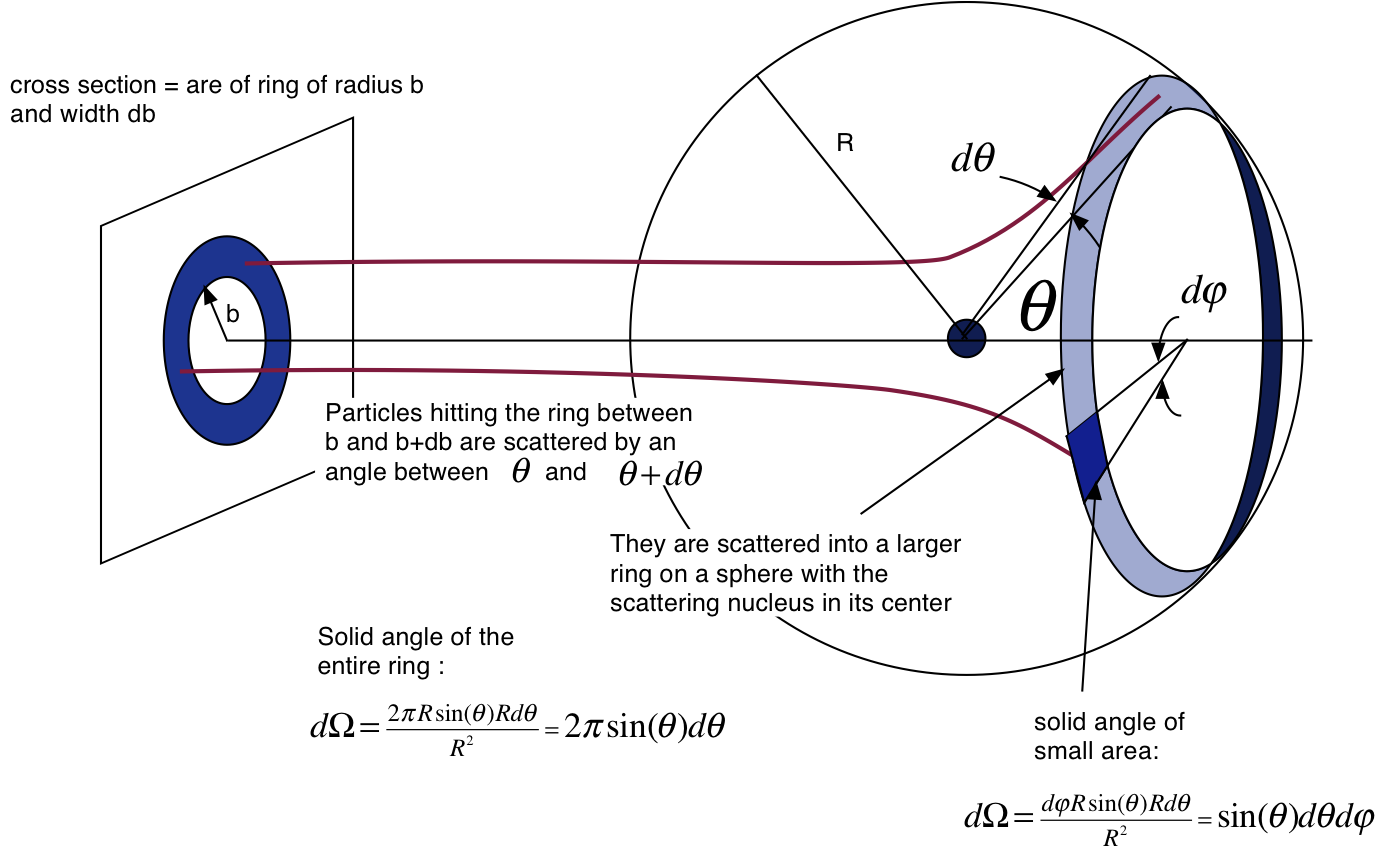
\includegraphics[width=0.95\textwidth]{rutherford.png}
	\caption{Sezione d'urto dello scattering di Rutherford.}
	\label{rutherford}
\end{figure}

Va notato che è possibile ignorare il fatto che la lamina target ha un numero elevato di atomi target e che ogni partiella nel beam incidente ha un diverso parametro d'urto relativo a ciascuno di essi, poiché la lastra è considerata così sottile da rendere improbabili collisioni multiple della stessa particella incidente; inoltre, dal modello atomico di Rutherford ricaviamo che i nuclei atomici si trovano a distanze grandi rispetto alle loro dimensioni, rendendo significative solo le traiettorie con parametro d'urto vicino al nucleo atomico.\\
Nel caso di un potenziale d'interazione generico, $ \Delta\sigma $ può avere anche dipendenza azimuthale:
\begin{equation}
	\Delta\sigma(\theta,\phi) = b \,db\,d\phi = - \frac{d\sigma}{d\Omega} (\theta,\phi) \,d\Omega= - \frac{d\sigma}{d\Omega} (\theta,\phi) \sin \theta \,d\theta\,d\phi
	\label{eq:6}
\end{equation}
dov'è stata utilizzata la differential cross-section $ \frac{d\sigma}{d\Omega} $ e dove si è tenuto conto che un aumento di $ b $ porta ad una diminuzione di $ \theta $ tramite il segno negativo.\\
Essendo il potenziale coulombiano un potenziale centrale a simmetria sferica, è possibile semplificare il calcolo grazie alla simmetria azimuthale, ottenendo:
\begin{equation}
	\frac{d\sigma}{d\Omega} (\theta) = - \frac{b}{\sin \theta} \frac{db}{d\theta}
	\label{eq:7}
\end{equation}
Lo scattering di Rutherford può essere quindi completamente caratterizzato utilizzando l'Eq. \ref{eq:5}:
\begin{equation}
	\frac{d\sigma}{d\Omega} (\theta) = \left( \frac{ZZ' e^2}{4 E_0} \right)^2 \frac{1}{\sin^2 \frac{\theta}{2}}
	\label{eq:8}
\end{equation}
È anche possibile definire la sezione d'urto totale $ \sigma_{\text{tot}} $ come:
\begin{equation}
	\sigma_{\text{tot}} = \int_{\Omega} \frac{d\sigma}{d\Omega} (\theta,\phi) \,d\Omega
	\label{eq:9}
\end{equation}
Essa rappresenta una sorta di area di scattering effettiva che la sorgente del potenziale determina a tutti i possibili valori del parametro d'urto.\\
Nel caso dello scattering di Rutherford:
\begin{equation}
	\begin{split}
		\sigma_{\text{tot}} &= \int_0^{2\pi} \int_0^{\pi} \frac{d\sigma}{d\Omega} (\theta,\phi) \sin \theta \,d\theta\,d\phi = 2\pi \int_0^{\pi} \frac{d\sigma}{d\Omega} (\theta) \sin \theta \,d\theta \\
				    &= 8\pi \left( \frac{ZZ' e^2}{4 E_0} \right)^2 \int_0^1 \frac{1}{\sin^3 \frac{\theta}{2}} d\left( \sin \frac{\theta}{2} \right) \longrightarrow \infty
	\end{split}
	\label{eq:10}
\end{equation}
Questo risultato divergente è coerente con l'interpretazione data della sezione d'urto totale: il potenziale coulombiano è associato all'interazione elettromagnetica, la quale ha un range infinito, dunque anche l'area efficace di scattering sarà infita.\\
In maniera realistica, però, si può considerare che dopo un determinato valore di cutoff $ b_0 $ lo scattering non abbia più effetti osservabili sulla particella incidente, dunque la sezione d'urto totale osservabile si ottiene integrando la differential cross-section tra $ 0 $ e $ \theta_0 < \pi$, ottenendo dunque un valore finito.\\
La formula di Rutherford \ref{eq:8} cessa di essere valida quando $ E_0 $ diventa troppo alta, in particolare quando la particella $ \alpha $ riesce a penetrare nel nucleo, poiché a quel punto subentrano l'interazione nucleare fin'ora ignorata: studiando sperimentalmente a quale energia (a differenti angoli di scattering) si iniziano a manifestare le deviazioni dalla cross-section di Rutherford, è possibile stimare il raggio nucleare tramite la distanza di closest approach $ a $, trovando il fit sperimentale $ R = R_0 A^{1/3} $ con $ R_0 = 1.4\fm $.

\subsection{Scattering elettronico}

Data la dualità onda-particella che risulta da una descrizione quanto-meccanica della materia, la sezione d'urto da scattering non sarà determinata soltanto dall'interazione coulombiana ma anche da effetti diffrattivi, evidenziati dal pattern di diffrazione in Fig. \ref{diffraction}: l'analogo ottico è la diffrazione da disco opaco, poiché il nucleo atomico assorbe nucleoni, con la dovuta differenza che la superficie del nucleo ha una determinata diffusività, la quale determina dei minimi non-nulli nello spettro di diffrazione.
\begin{figure}
	\centering
	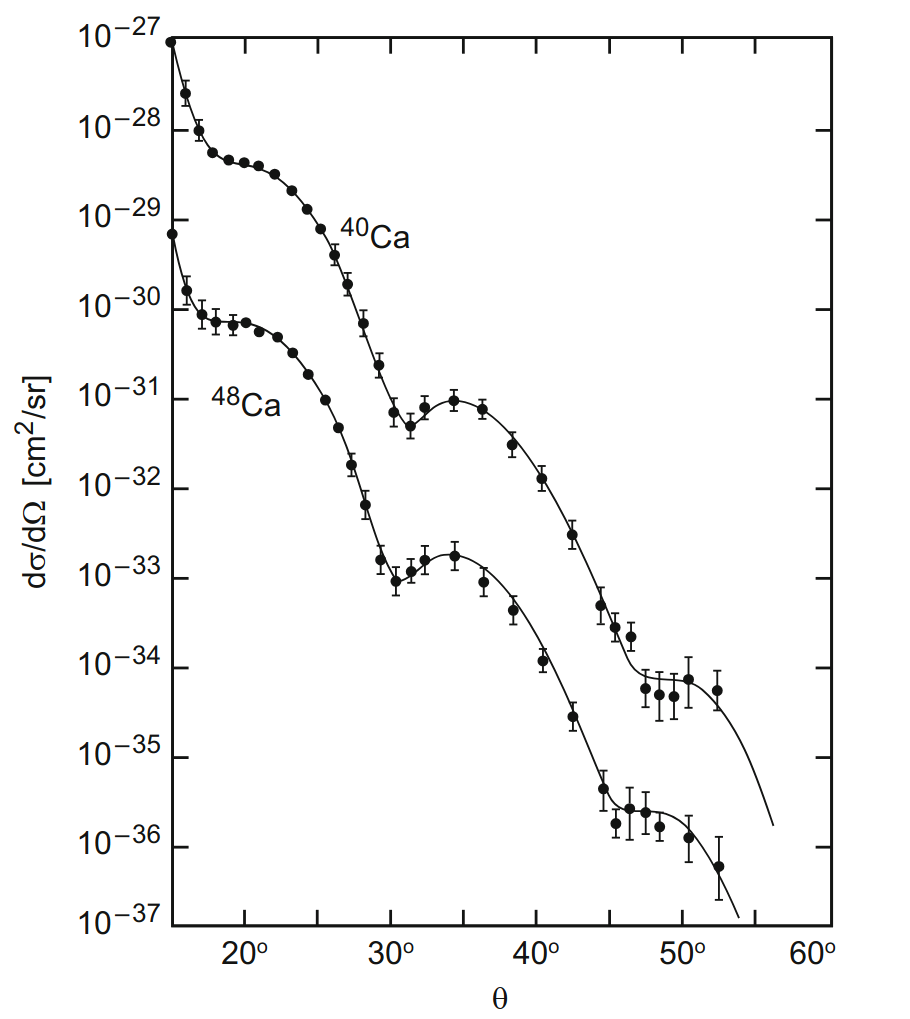
\includegraphics[width=0.95\textwidth]{diffraction.png}
	\caption{Sezione d'urto dello scattering elettronico.}
	\label{diffraction}
\end{figure}\\
Per evitare che all'interazione coulombiana si sovrapponga anche quella tra nucleoni, per studiare la struttura del nucleo atomico le sonde migliori sono gli elettroni: poiché per sondare una scala di lunghezze $ \Delta x $ è necessaria una lunghezza d'onda $ \lambda \sim \Delta x $, dalla relazione di de Broglie si ha che la quantità di moto degli elettroni incidenti deve essere $ p \sim h / \Delta x $. La struttura del nucleo atomico risulta visibile su scale di $ 1\fm $, dunque sono necessari elettroni con momento lineare $ p \approx 200 \mev/c $; nel caso si voglia studiare la struttura interna dei nucleoni, la stima aumenta di almeno un ordine di grandezza.\\
Va ricordato che gli elettroni, in quanto particelle cariche, quando percorrono una traiettoria curva irraggiano, dunque per questo tipo di scattering sono necessari accelleratori lineari.
Ricordando che $ E^2 = p^2 c^2 + m_0^2 c^4 $ ed $ E = K + m_0 c^2 $, considerando che $ m_e = 0.511 \mev/c^2 $, si vede che gli elettroni utilizzati per sondare il nucleo atomico sono in regime ultra-relativistico, dunque nel calcolo della cross-section sono da tenere in conto effetti relativistici legati allo spin ed il nuclear recoil (ovverosia il rinculo subito dal nucleo atomico a seguito dello scattering): trascurando quest'ultimo, si può applicare una correzione alla cross-section di Rutherford, detta cross-section di Mott:
\begin{equation}
	\left(\frac{d\sigma}{d\Omega}\right)_{\text{Mott}} = \left(\frac{d\sigma}{d\Omega}\right)_{\text{Ruth}} \left(1 - \beta^2 \sin^2 \frac{\theta}{2}\right)
	\label{eq:11}
\end{equation}
Queste sezioni d'urto, però, considerano scattering tra oggetti puntiformi, ma mentre un elettrone può effettivamente essere considerato tale, lo stesso non si può dire per il nucleo atomico, il quale avrà una certa distribuzione di carica $ \rho(\ve{r}) $ estesa nello spazio (essa coincide con la distribuzione di massa solo per nuclidi stabili); per considerare anche questo fatto, nel calcolo della cross-section si applica un'ulteriore correzione:
\begin{equation}
	\frac{d\sigma}{d\Omega} = \left(\frac{d\sigma}{d\Omega}\right)_{\text{Mott}} \abs{F(q)}^2
	\label{eq:12}
\end{equation}
dove $ \abs{F(q)}^2 $ è detto form factor e $ \ve{q} \defeq \frac{1}{\hbar} \abs{\ve{p}' - \ve{p}} $, con $ \ve{p} $ e $ \ve{p}' $ momento iniziale e finale dell'elettrone, esprime la variazione di quantità di moto dell'elettrone.\\
Dato che si sta considerando uno scattering elastico, si ha $ p = p' $ e dunque $ q = \frac{1}{\hbar} 2p \sin \frac{\theta}{2} $, con $ \theta $ angolo di scattering.\\
Nel caso dell'approssimazione di Born (elettroni come onde piane $ \psi(\ve{r}) = \frac{1}{\sqrt{V}} e^{i \ve{p}\cdot\ve{x} / \hbar} $) e trascurando il nuclear recoil, il form factor è la trasformata di Fourier della distribuzione di carica $ \rho(\ve{r}) $:
\begin{equation}
	F(q) = \int_{r \le R} e^{i \ve{p}\cdot\ve{r} / \hbar} \rho(\ve{r}) d^3\ve{r}
	\label{eq:13}
\end{equation}
con $ R $ raggio nucleare ed opportuna normalizzazione $ F(0) = 1 $.\\
In questa approssimazione, quindi, una misura della cross-section di scattering elettronico può dare informazioni sulla distribuzione di carica nel nucleo atomico; inoltre, è possibile dare una stima del raggio nucleare dallo studio dello spettro di diffrazione evidenziato dalla cross-section, poiché il primo minimo di diffrazione soddisfa la relazione $ \frac{q}{\hbar} \approx \frac{4.5}{R} $; se invece si considerano due isotopi, dal fatto che la separazione angolare tra due minimi è $ \Delta\theta = \frac{\hbar}{p R} $ si evince che all'aumentare del numero di massa aumenta anche il raggio nucleare (vedere Fig. \ref{diffraction}): ciò in generale è valido solo per nuclidi nella cosiddetta $ \virgolette{valle di stabilità} $, poiché per essi la distribuzione di neutroni segue quella di protoni, ovvero le distribuzioni ci carica e massa vanno a coincidere, dunque un nuclide con più nucleoni avrà un raggio nucleare maggiore; la difficoltà principale nella misura della distribuzione di nucleoni sta nel fatto che i neutroni sono trasparenti agli esperimenti di scattering, poiché non interagiscono né tramite interazione elettromagnetica né tramite interazione nucleare forte.

\subsubsection{Distribuzione di carica nucleare}

Compiendo esperimenti di scattering elettronico e raccogliendo dati relativi a vari nuclei atomici, si è giunti alla conclusione che i nuclidi non sono sfere con un confine ben delineato, ma al loro interno la densità di carica si mantiene approssimativamente costante, mentre verso la superficie essa si riduce su un intervallo radiale relativamente ampio; la distribuzione di carica nucleare può dunque essere approssimata da una distribuzione di Fermi:
\begin{equation}
	\rho(\ve{r}) = \frac{\rho_0}{1 + e^{(r - c) / a}}
	\label{eq:14}
\end{equation}
dove i parametri empirici valgono (per nuclei pesanti) $ c = 1.07\fm \cdot A^{1/3} $ e $ a = 0.54\fm $: $ c $ è il raggio nucleare a mezza altezza della distribuzione di carica, mentre $ a $ è la diffusività (ciò che rende la distribuzione smooth piuttosto che sharp).\\
Una volta nota la distribuzione di carica, è possibile calcolare il raggio quadratico medio: per nuclei medi e pesanti, si ha $ \sqrt{\langle r^2 \rangle} = 0.94\fm \cdot A^{1/3} $. Se si approssima il nucleo come una sfera uniformemente carica, il suo raggio, definito come raggio nucleare, è dato da $ R^2 = \frac{5}{3} \langle r^2 \rangle $, ovvero:
\begin{equation}
	R = 1.21\fm \cdot A^{1/3}
	\label{eq:14-bis}
\end{equation}
che è la definizione più diffusa di raggio nucleare.\\
È anche possibile definire una skin depth (o surface thickness) $ t $ come lo spessore del guscio sferico in cui la densità di carica diminuisce dal $ 90\% $ al $ 10\% $ del suo valore massimo: per nuclei pesanti, si trova $ t = 2a\ln9 \approx 4.4 a $.\\
Come si può vedere in Fig. \ref{charge-distr}, la densità di carica centrale $ \rho_0 $ diminuisce leggermente all'aumentare del numero di massa; se però viene considerata la presenza di neutroni e si moltiplica per un fattore $ A / Z $, si trova un valore quasi identico per tutti i nuclidi (questo è coerente con $ R \sim A^{1/3} $, poiché così $ \rho_0 \sim A / \text{Vol} $ rimane costante): questo corrisponde alla densità che teoricamente avrebbe della materia nucleare infinitamente estesa, pari a $ \rho_n \approx 0.17 \,\text{nucleoni} / \text{fm}^3 $, che corrisponde a $ c = 1.12\fm \cdot A^{1/3} $.
\begin{figure}[!ht]
	\centering
	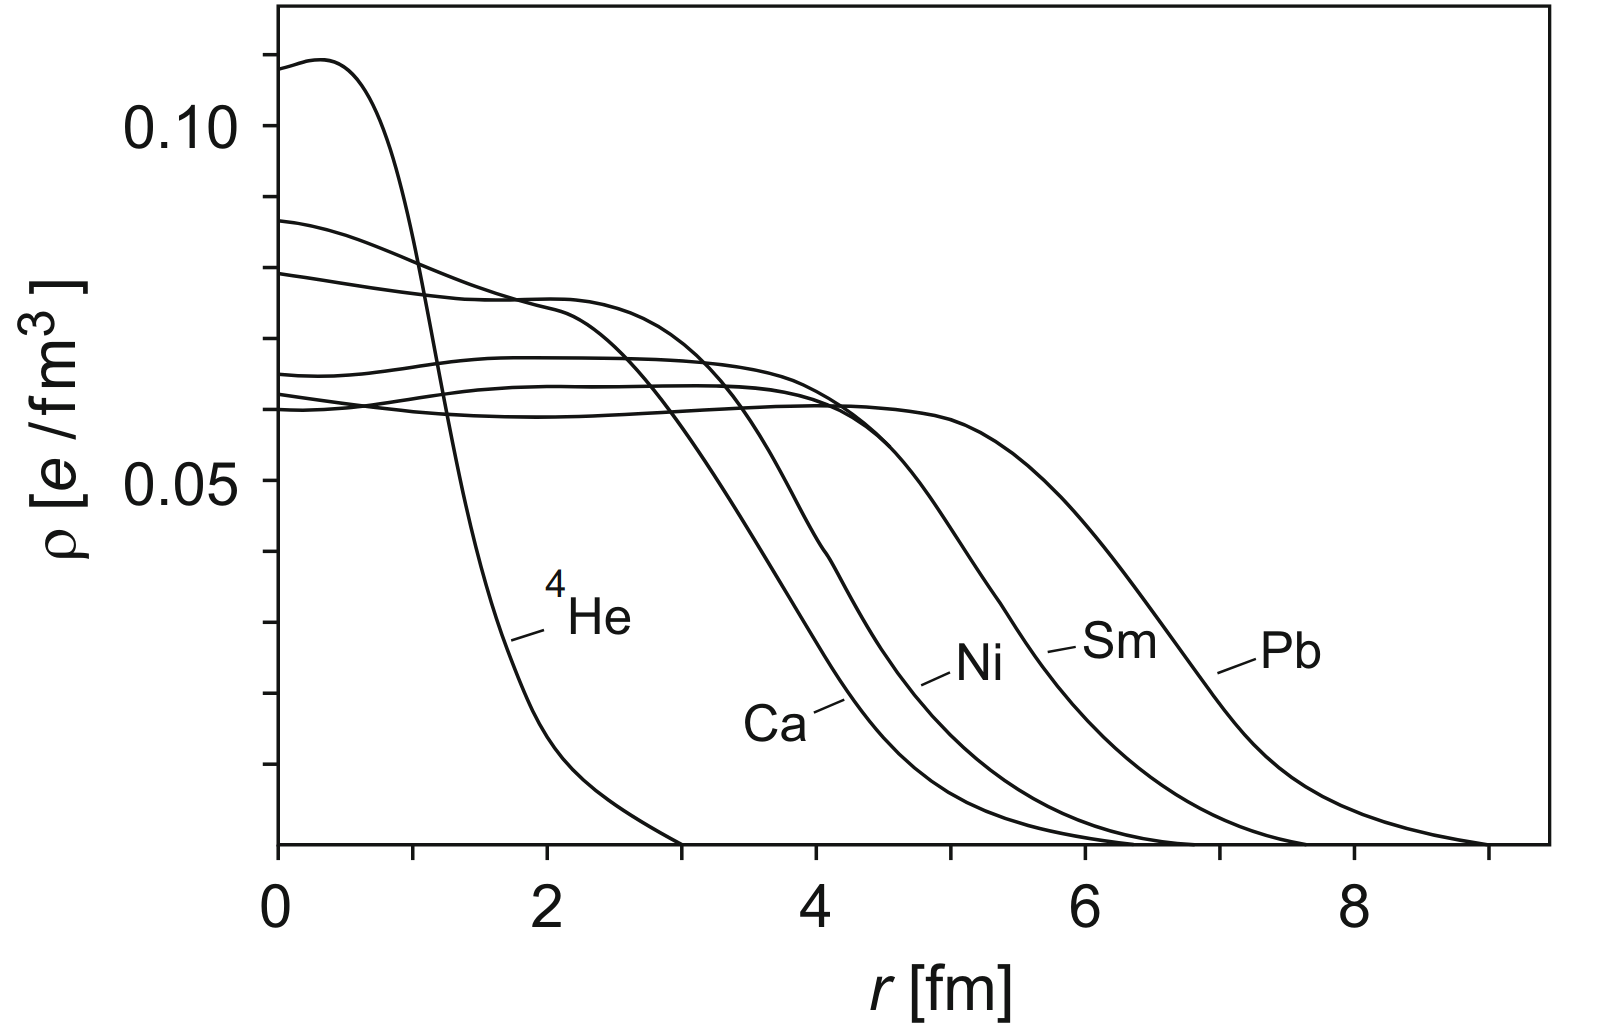
\includegraphics[width=0.95\textwidth]{charge-distribution.png}
	\caption{Distribuzione di carica in vari nuclidi.}
	\label{charge-distr}
\end{figure}

Sperimentalmente si trova che alcuni nuclidi (ad esempio i lantanidi) non hanno una forma sferica ma assumono deformazioni ellissoidali: queste forme non possono essere studiate con scattering elettronico, poiché esso evidenzia soltanto una superficie molto diffusa.\\
Va infine notato che nuclidi leggeri come $ \ch{^{6,7}Li} $, $ \ch{^{9}Be} $ e soprattutto $ \ch{^{4}He} $ costituiscono dei casi speciali: essi non presentano una densità di carica centrale costante, ma il suo andamento è approssimativamente gaussiano.

\subsubsection{Nuclidi instabili}

Quanto riportato fin'ora vale solo per nuclidi nella valle di stabilità (vedere Fig. \ref{segre-chart}), ovverosia l'insieme di nuclei stabili che non decadono radioattivamente (tipicamente per decadimento $ \beta $), i quali sono osservati in abbondanza sulla Terra.\\
Se, partendo dalla valle di stabilità, si percorre una catena isotopica, i nuclidi diventano via via più neutron-rich, fino a quando non si raggiungono le driplines, oltre le quali i nuclei non sono più sistemi legati a causa dell'interazione nucleare forte.\\
Lo spostamento verso nuclidi esotici neutron-rich causa un mutamento drastico rispetto ai loro isotopi stabili: in un lavoro pionieristico del 1985 di Tanihata et al., fu misurata la cross-section d'interazione tra nuclei di $ \ch{^{11}Li} $ (isotopo instabile) e dei nuclidi stabili target, la quale può essere teoricamente calcolata dal modello di Glauber per lo scattering relativistico di nuclidi (traiettorie iniziali e finali rettilinee) come $ \sigma_I \sim \pi \left( R_p^2 + R_t^2 \right) $, dove $ R_p $ è il raggio del nucleo proiettile ed $ R_t $ quello del nucleo target; dai dati fu possibile ricavare il raggio nucleare del $ \ch{^{11}Li} $, il quale dovrebbe essere dell'ordine di $ \sim 2.4\fm $, trovando un valore cinque volte maggiore (comparabile con quello del $ \ch{^{208}Pb} $): questa fu la prima verifica sperimentale dell'esistenza di sistemi ad alone, nuclidi con un corpo centrale sferico circondati da uno o due neutroni o protoni (si parla di neutron skin o proton skin), i quali vanno a formare un halo attorno al nucleo aumentandone considerevolmente le dimensioni osservate.\\
Condurre esperimenti di scattering elettronico su nuclei instabili è estremamente difficile, poiché pochi di essi hanno delle vite medie abbastanza lunghe, dunque non è possibile predisporre un target composto del materiale da studiare: in alcuni laboratori si è riusciti a costruire delle trappole con le quali i nuclidi instabili sono accellerati e confinati, così da poter essere bombardati da fasci elettronici.

\paragraph{Luminosità}

Nello studio dei rilevatori di scattering un importante parametro è la luminosità:
\begin{equation}
	\mathcal{L} = N_b N_t
	\label{eq:15}
\end{equation}
dove $ N_b $ è il numero di particelle incidenti per unità di tempo e $ N_t $ il numero di nuclidi target per unità d'area.\\
Questo parametro è legato all'efficienza del rilevatore, misurata dal numero di eventi rilevati nell'unità di tempo $ \dot{N} $:
\begin{equation}
	\dot{N} (E, \theta) = \mathcal{L}\, \frac{d\sigma}{d\Omega} (E,\theta) \,\Delta\Omega
	\label{eq:16}
\end{equation}
Nel caso dello scattering elettronico, la cross-section è molto piccola, dunque sono necessari collisori dall'elevata luminosità (tecnicamente difficile): si va da $ \mathcal{L}_{\text{min}} \sim 10^{26} \,\text{cm}^{-2} \,\text{s}^{-1} $ per sondare nuclidi con $ Z \sim 80 $ a $ \mathcal{L}_{\text{min}} \sim 10^{31} \,\text{cm}^{-2}\,\text{s}^{-1} $ per $ Z \sim 10 $.\\
Inoltre, la luminosità varia anche in base al target considerato: per nuclidi stabili si raggiungono luminosità per scattering elettronico di $ 10^{33} \,\text{cm}^{-2}\,\text{s}^{-1} $ (es: STABLE), mentre su nuclidi instabili si arriva a $ 10^{27} \,\text{cm}^{-2}\,\text{s}^{-1} $ (es: SCRIT).

\section{Proprietà dei nuclidi}

\subsection{Masse nucleari}

Preso un atomo di una specie chimica $ ^A_Z \text{X}_N $, se si sommano le masse degli $ N $ neutroni, dei $ Z $ protoni e dei $ Z $ elettroni, si trova una massa minore di quella misurata per l'atomo: questo avviene poiché, essendo l'atomo uno stato legato, parte della massa dei suoi costituenti viene convertita in energia di legame (positiva, poiché stato legato), ovvero:
\begin{equation}
	M_{\text{atom}} = N m_n + Z \left( m_p + m_e \right) - \frac{1}{c^2} \left( B_{\text{atom}} + B_{\text{nucleus}} \right)
	\label{eq:1.17}
\end{equation}
dove si è distinto tra binding energy atomica e nucleare: queste ultime sono conosciute con incertezze maggiori, dato che $ (\delta m / m)_{\text{atom}} \sim 10^{-10} $ e $ (\delta m / m)_{\text{nucleus}} \sim 10^{-7} $.\\
Si trova quindi che la binding energy di un nuclide può essere espressa come:
\begin{equation}
	B(A,Z) = \left[ Z m({\ch{^{1}H}}) + N m_n - M(A,Z) \right] c^2
	\label{eq:1.18}
\end{equation}
dove si sono usate le masse atomiche, poiché misurate con più precisione (si ricordi la conversione $ 1u \approx 931.494\mev/c^2 $).\\
La misura delle masse atomiche è importante poiché permette di fare misure indirette sulle masse nucleari, e dunque studiare l'abbondanza isotopica di un elemento, e di stimare le binding energies, le quali sono legate alla natura della forza nucleare.\\
Ci sono varie tecniche per misurare le masse atomiche: spettrometri di massa, cinematica delle reazioni (solitamente quando i primi non si possono utilizzare), trappole (ad oggi gli strumenti più precisi) ed anelli di accumulazione (storage rings).

\subsubsection{Spettrometri di massa}

Uno spettrometro di massa permette di misurare le masse di ioni di un determinato elemento.
\begin{figure}[!b]
	\centering
	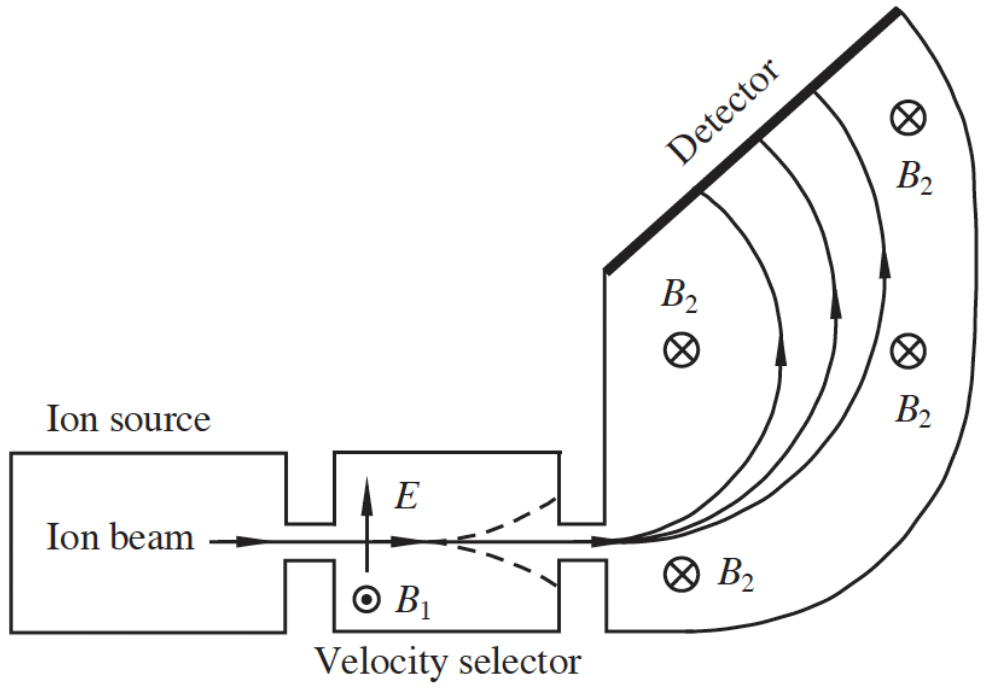
\includegraphics[width=0.75\textwidth]{spectrometer.png}
	\caption{Schematizzazione di uno spettrometro di massa.}
	\label{spettr}
\end{figure}

Schematicamente (Fig. \ref{spettr}), esso è costituito da:
\begin{itemize}
	\item una sorgente di ioni;
	\item un selettore di velocità;
	\item uno spettrometro magnetico;
	\item un focal plane detector.
\end{itemize}
La sorgente di ioni ionizza gli atomi da studiare, li accellera e li collima in un fascio; questo fascio viene diretto in un selettore di velocità: questo è solitamente un filtro di Wien, composto da un campo elettrico e un campo magnetico incrociati che determinano traiettorie rettilinee solo se $ \ve{F}_E + \ve{F}_B = \ve{0} $, ovvero, assumendo un fascio già collimato nella direzione desiderata, se $ v = E / B $.\\
L'elemento ottico di questo setup è lo spettrometro magnetico: in esso le traiettorie degli ioni curvano in base al loro momento e alla loro carica, dato che il raggio di girazione è $ r = \frac{vm}{qB} $: di conseguenza, sperimentalmente vanno misurati sia il raggio di girazione che la carica per poter determinare la massa dello ione, e ciò è proprio quello che fa il focal plane detector.\\
Va notato che, in generale, le misure assolute di massa non permettono una grande precisione, perciò si preferisce effettuare misurazioni rispetto a ioni di cui già di conosce bene la massa: in particolare, le precisioni maggiori si raggiungono sui mass ratios tra ioni di egual carica, poiché in tal caso $ m_1 / m_2 = r_1 / r_2 $. Il campione di riferimento solitamente utilizzato è il carbonio, poiché dati i suoi numerosi composti permette di effettuare misure su un vasto range di ioni.

\paragraph{Abbondanze isotopiche}

Tendenzialmente, un elemento avrà più di un isotopo stabile (if any at all), dunque con una spettrografia di massa risulterà una distribuzione di massa con picchi di abbondanza relativa corrispondenti agli isotopi stabili: ciò permette di misurarne le masse $ m_i $ e l'abbondanza percentuale nel campione $ w_i $, così da poter stimare la massa atomica dell'elemento come media ponderata $ m = \sum_{i} w_i m_i $.\\
In generale, le abbondanze isotopiche sono diverse nell'Universo rispetto alla Terra, ed anche sulla Terra possono avere forti fluttuazioni tra una zona geografica e l'altra; ad esempio, si considerino due campioni di $ \ch{Xe} $, uno prelevato da una roccia metamorfica vecchia di $ 2.7 \text{Gy} $ ed uno dall'atmosfera: le relative analisi spettrografiche (riportate in Fig. \ref{iso-distr}) mostrano delle diverse abbondanze isotopiche nei due campioni, dovute alla presenza nella roccia metamorfica di prodotti della fissione nucleare spontanea dell'uranio.
\begin{figure}[!b]
	\centering
	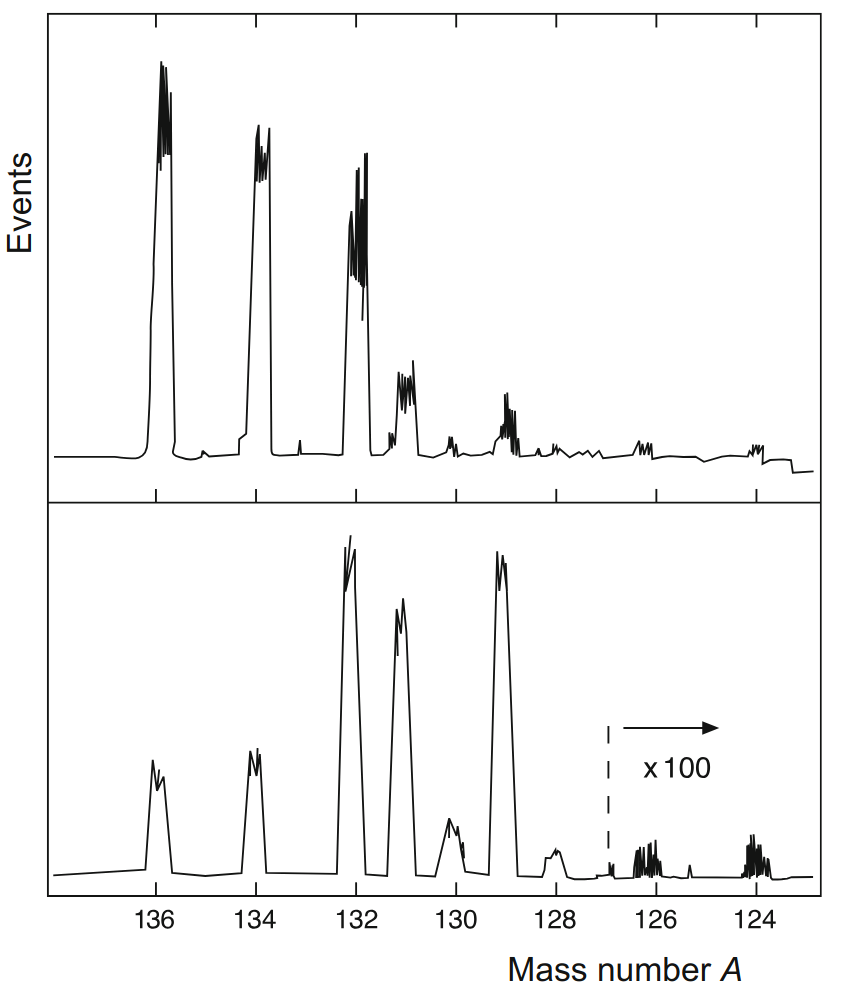
\includegraphics[width=0.55\textwidth]{isotop-distr.png}
	\caption{Distribuzioni isotopiche di due campioni di $ \ch{Xe} $, il primo prelevato da una roccia metamorfica, il secondo dall'atmosfera.}
	\label{iso-distr}
\end{figure}

\begin{figure}[!ht]
	\centering
	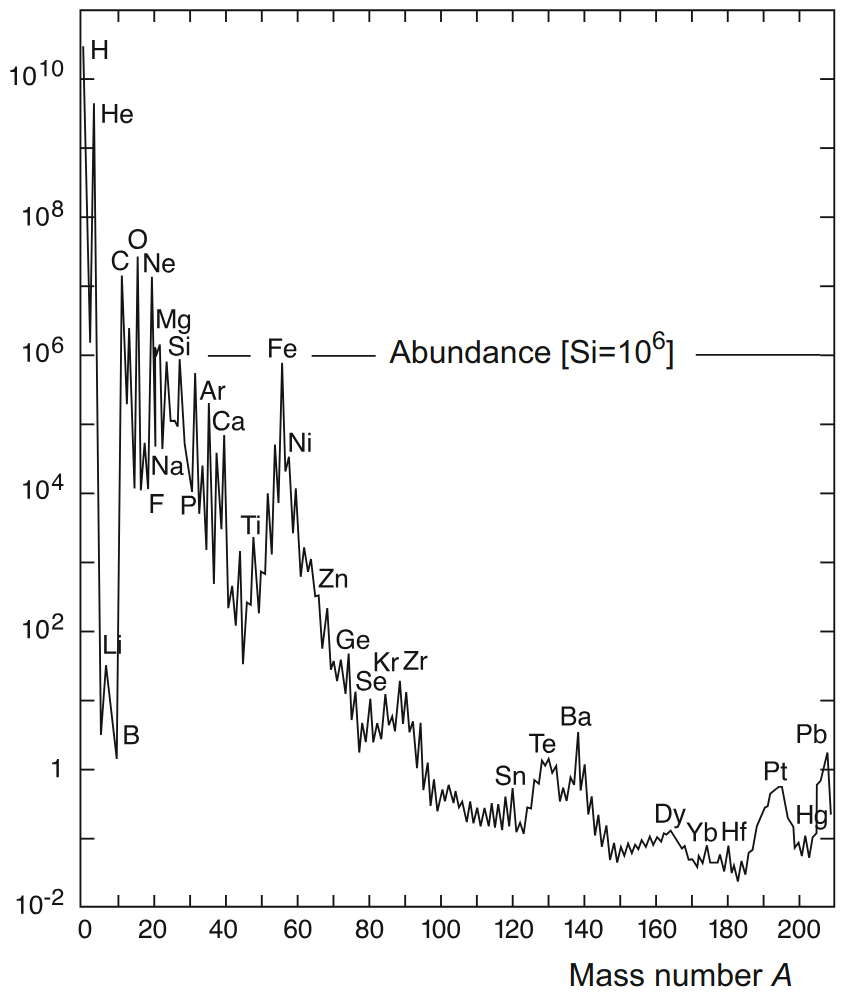
\includegraphics[width=0.75\textwidth]{isotop-distr-univ.png}
	\caption{Distribuzioni isotopiche dei principali elementi nel Sistema Solare, normalizzati all'abbondanza del $ \ch{Si} $: l'abbondanza del $ \ch{Li} $ è uno dei problemi nella ricostruzione dell'origine dell'Universo.}
	\label{iso-distr-univ}
\end{figure}
Lo studio delle abbondanze relative nell'Universo (Fig. \ref{iso-distr-univ}) permette di studiarne l'evoluzione: secondo gli attuali modelli, la sintesi di deuterio ed elio è avvenuta all'origine dell'Universo dalla fusione nucleare dell'idrogeno, mentre i nuclidi fino al $ \ch{^{56}Fe} $ vengono sintetizzati dalla fusione nucleare nei nuclei stellari; per quanto riguarda i nuclei pesanti, invece, la loro sintesi avviene nelle esplosioni di stelle molto massive.

\subsubsection{Cinematica delle reazioni}

Qualora il tempo di volo tra il generatore di ioni ed il piano focale fosse maggiore della vita media dello ione che si vuole studiare, al posto della spettroscopia di massa è possibile calcolare la massa dello ione studiandone le sue reazioni.\\
Si consideri una reazione del tipo:
\begin{equation}
	a + \text{X} \longrightarrow b
	\label{eq:1.19}
\end{equation}
dove $ a $ è la particella proiettile, $ \text{X} $ lo ione target e $ b $ rappresenta l'insieme di prodotti della reazione.\\
Assumendo uno scattering elastico, la conservazione dell'energia ci dà:
\begin{equation}
	m_a c^2 + T_a + m_{\text{X}} c^2 + T_{\text{X}} = m_b c^2 + T_b
	\label{eq:1.20}
\end{equation}
È possibile definire il cosiddetto Q-value della reazione:
\begin{equation}
	Q \defeq T_{\text{final}} - T_{\text{initial}} = T_b - T_a - T_{\text{X}}
	\label{eq:1.21}
\end{equation}
così da poter calcolare la massa dell'isotopo $ \text{X} $ come:
\begin{equation}
	m_{\text{X}} = \frac{1}{c^2} Q + m_b - m_a
	\label{eq:1.22}
\end{equation}
Con questo metodo, è possibile raggiungere una precisione $ \delta m / m \sim 10^{-6} $.

\subsubsection{Trappole}

Le trappole sono dispositivi in grado di confinare ioni grazie a campi elettromagnetici finemente controllati. Esse vengono usate soprattutto quando la vita media dello ione radioattive non permette l'utilizzo né di spettrometri di massa (a causa del tempo di volo) né di reazioni cinematiche (per sezioni d'urto bassissime).\\
Il vantaggio delle trappole è che permettono lo studio prolungato anche di singoli radioisotopi in regimi energetici bassissimi, dunque con velocità pressoché nulle, limitatamente alle loro vite medie.\\
Sebbene le trappole abbiano incertezze relative bassissime ($ \delta m / m \sim 10^{-8} $ per nuclidi instabili e $ 10^{-11} $ per nuclidi stabili), in determinati si sceglie di usare gli anelli di accumulazione poiché, nonostante le incertezze leggermente più alte, permettono di raggiungere energie relativistiche, rendendo possibili misurazioni su isotopi con vite medie cortissime.

\paragraph{Trappola di Penning}

Una trappola costituita da 4 elettrodi pensata per isotopi prodotti con velocità basse (principalmente tecnica ISOL\footnote{Ioni incidono su una lastra di carbonato di uranio a $ 4000\cels$ così da poter effondere e diffondere attraverso la superficie con un'energia cinetica bassissima; sono possibili anche tecniche di accellerazione e post-accellerazione.}), i quali vengono confinati radialmente da un campo magnetico (per moto di ciclotrone) ed assialmente da un campo elettrostatico di quadrupolo.\\
Il moto all'interno della trappola è molto complicato, poiché somma di un moto di magnetone circolare attorno all'asse di $ \ve{B} $ con frequenza $ \omega_- $, un moto di ciclotrone spiraleggiante attorno alle linee di $ \ve{B} $ con frequenza $ \omega_+ $ ed un moto oscillatorio longitudinale determinato da $ \ve{E}_{\text{quad}} $ con frequenza $ \omega_z $. Si dimostra il seguente teorema d'invarianza:
\begin{equation}
	\omega_c^2 = \omega_+^2 + \omega_-^2 + \omega_z^2
	\label{eq:1.23}
\end{equation}
Ciò permette di misurare la massa dello ione, ricordando che la frequenza di ciclotrone è $ \omega_c = \frac{q B}{m} $.\\
Le misure effettuate sono sempre misurazioni relative di massa (solitamente con campione $ \ch{^{12}C} $), così da includere eventuali errori sistematici.

\subsubsection{Anelli di accumulazione}

Un anello di accumulazione è un accelleratore di particelle circolare in cui un fascio di ioni viene fatto circolare a velocità relativistica per un periodo prolungato di tempo.\\
Gli ioni vengono prodotti con velocità relativistiche (principalmente tecnica in flight\footnote{Nuclei radioattivi (es: $ \ch{^{238}U} $) vengono accellerati a diverse centinaia di MeV per nucleone e fatti scontrare su target di $ \ch{^{9}Be} $, frammentandosi in prodotti con velocità relativistiche, i quali vengono poi selezionati da strumenti ottici in base al rapporto $ m/q $.}) ed immessi nell'anello; la loro massa è determinata dal periodo di rivoluzione:
\begin{equation}
	\frac{\Delta T}{T} = \frac{1}{\gamma_t^2}\frac{\Delta (m/q)}{m/q} - \left( 1 - \frac{\gamma^2}{\gamma_t^2} \right) \frac{\Delta v}{v}
	\label{eq:1.24}
\end{equation}
Il secondo termine è una correzione dovuta alla transition energy (il valore per cui l'energia diventa indipendente dalla specie chimica nell'anello) e alla dispersione delle velocità, ed è eliminabile tramite tecniche ingegneristiche: in particolare, esistono anelli di accumulazione progettati col metodo di Schottky (cool fragments), per i quali $ \frac{\Delta v}{v} \rightarrow 0 $, e quelli a traiettorie isocrone (hot fragments, così da avere energia pari all'energia di transizione), per i quali $ \gamma_t \rightarrow \gamma $. Con questi anelli di accumulazione si raggiunge $ \delta m / m \sim 10^{-8} $.

\subsection{Binding energy}

Riprendendo l'Eq. \ref{eq:1.18}, si definisce la binding energy di un nuclide $ ^A_Z \text{X}_N $ come:
\begin{equation}
	B(A,Z) = \left[ Z m({\ch{^{1}H}}) + N m_n - M(A,Z) \right] c^2
	\label{eq:1.25}
\end{equation}
La binding energy è positiva nel caso di nuclidi legati, ovvero quelli che possono effettivamente esistere nel loro stato fondamentale (anche se con vite medie corte).\\
Come si può vedere in Fig. \ref{bind-en}, se si restringe l'analisi ai nuclidi stabili e long-lived, si nota che, a seguito di rapide variazioni per bassi $ A $, la binding energy per nucleone si stabilizza a circa $ 8\mev/\text{nucleone} $ per i pesanti (oltre il $ \ch{^{56}Fe} $): i nuclei più stabili sono $ \ch{^{62}_{28}Ni} $, $ \ch{^{58}_{26}Fe} $ e $ \ch{^{56}_{26}Fe} $.
\begin{figure}
	\centering
	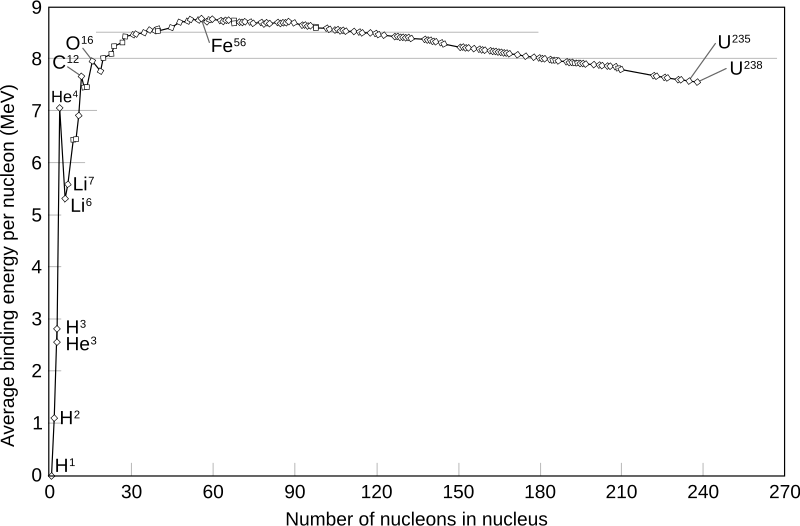
\includegraphics[width=0.75\textwidth]{bind-en.png}
	\caption{Binding energy table for stable and long-lived nuclei.}
	\label{bind-en}
\end{figure}

Sempre dal grafico in Fig. $ \ref{bind-en} $ è possibile fare alcune considerazioni:
\begin{enumerate}
	\item i nuclei pari-pari (numero pari di neutroni e di protoni) sono energeticamente favoriti rispetto a quelli pari-dispari, poiché più legati (es: $ \ch{^{4}He} $ è il nuclide leggero più legato), inoltre non ci sono nuclidi stabili per $ A = 5,8 $;
	\item il rapporto $ B/A \sim 8\mev $ costante per i nuclei pesanti evidenzia la natura a corto raggio dell'interazione forte, la quale viene saturata (un nucleone risente solo dei nucleoni vicini);
	\item il picco attorno ad $ A \sim 60 $ mostra come, tendendo all'equilibrio, i nuclidi leggeri guadagnano energia formando nuclei più pesanti tramite fusione nucleare (es: ambiente stellare), mentre i nuclidi pesanti perdono energia separandosi in nuclei leggeri tramite fissione nucleare.
\end{enumerate}
È necessario fare una precisazione: un nuclide può essere legato ma comunque instabile. Ad esempio, il $ \ch{^8 Be} $ ha $ B = 56.5\mev $, ma rispetto al decadimento $ \alpha $ si ha $ \ch{^8 Be} \rightarrow 2\alpha $, il quale ha una variazione d'energia $ B_{\text{decay}} = - 0.092\mev $: si evince che nel suo stato fondamentale il $ \ch{^8 Be} $ non esiste in uno stato legato, ma come risonanza di due particelle $ \alpha $, la quale sussiste per un certo periodo di tempo prima di decadere.\\
In generale, se esiste almeno una combinazione di neutroni e protoni non legata, allora il nuclide allo stato fondamentale non esiste in uno stato legato e decade; inoltre, di solito sono possibili varie modalità di decadimento, dette decay branches.

\subsubsection{Formula semi-empirica di Weizsäcker}

È possibile dare un'interpretazione fenomenologica della binding energy tramite un modello semplificato del nucleo atomico: il modello a goccia. Questo modello si basa sulle seguenti ipotesi:
\begin{enumerate}
	\item l'energia d'interazione tra due nucleoni è indipendente dal tipo e dal numero di nucleoni (non si distingue tra neutroni e protoni);
	\item l'interazione tra nucleoni è attrattiva a breve raggio per $ r < R_{\text{int}} $ e repulsiva a brevissimo raggio per $ r \ll R_{\text{int}} $;
	\item la binding energy del nucleo è proporzionale al numero di nucleoni (e dunque al volume del nucleo).
\end{enumerate}
Questo modello implica delle forze sature tra nucleoni, in cui ciascuno nucleone è legato solo ai nucleoni immediatamente vicini; definendo l'energia d'interazione tra due nucleoni $ \langle U \rangle $, ciò implica che la binding energy del nucleo non è data dalla somma di tutte le coppie di nucleoni, ma solo delle coppie vicine in un volume $ V_{\text{int}} < V_{\text{nucleo}} $. Ricordando che $ V_{\text{nucleo}} \sim A $, si ha:
\begin{equation}
	B_0 = \sum_{r < R_{\text{int}}} U = \frac{A(A-1)}{2}\langle U \rangle \frac{V_{\text{int}}}{V_{\text{nucleo}}} \sim b_0 A
	\label{eq:1.26}
\end{equation}
A questa stima cruda vanno aggiunti dei termini correttivi per effetti di cui il modello a goccia non tiene conto.\\
Innanzitutto, va considerato un termine di superficie, dovuto al fatto che i nucleoni sulla superficie del nucleo interagiscono con un minor numero di nucleoni, dunque sono meno legati; dato che il raggio atomico è $ R \sim A^{1/3} $, il termine di superficie va come $ B_{\text{sup}} \sim - b_1 A^{2/3} $.\\
Bisogna anche considerare la repulsione coulombiana tra protoni, la quale può essere approssimata col modello della sfera uniformemente carica (dai form factors, $ \rho $ è circa costante all'interno del nucleo):
\begin{equation}
	 U_e = \int_0^R V(r) \rho(r) 4\pi r^2 dr = \int_0^R \frac{Ze}{4\pi \epsilon_0 r} \left( \frac{r}{R} \right)^3 \frac{Ze}{\frac{4}{3}\pi R^3} 4\pi r^2 dr = \frac{3}{5} \frac{(Ze)^2}{4\pi \epsilon_0 R}
	\label{eq:1.27}
\end{equation}
Dunque va aggiunta una correzione $ B_{\text{Coulomb}} \sim - b_2 \frac{Z^2}{A^{1/3}} $.\\
Essendo il nucleo un sistema quantistico, è naturale che nella sua descrizioni siano inclusi gli effetti quantistici: in particolare, il calcolo dell'energia cinetica dei nucleoni può essere svolto prendendo come modello un gas di Fermi, il quale tiene conto della statistica dei fermioni e del principio di esclusione di Pauli (questo favorisce la formazione di nuclei con egual numero di protoni e neutroni); l'energia cinetica totale risulta essere:
\begin{equation}
	K_{\text{tot}} \approx 20 \mev \left( A + \frac{5}{9} \frac{(N - Z)^2}{A} \right)
	\label{eq:1.28}
\end{equation}
Il primo termine si aggiunge al termine di volume $ B_0 $, mentre il secondo termine determina un termine correttivo $ B_{\text{sym}} \sim - b_3 \frac{(N - Z)^2}{A} $.\\
Infine, lo studio delle masse nucleari mostra che i nuclei con un numero pari di protoni e/o neutroni sono più stabili: ciò viene interpretato come un accoppiamento a doppietti sia dei protoni che dei neutroni (in base ai loro spin e momento angolare, in modo da avere spin totale nullo). Empiricamente, ciò determina un fattore correttivo alla binding energy pari a:
\begin{equation}
	B_{\text{parity}} \sim - \delta A^{-1/2}, \qquad \delta =
	\begin{cases}
		+11.2\mev & \text{dispari-dispari} \\
		0\mev & \text{dispari-pari o pari-dispari} \\
		-11.2\mev & \text{pari-pari}
	\end{cases}
	\label{eq:1.29}
\end{equation}
Si è sostanzialmente ricavata la \textit{formula semi-empirica di Weizsäcker}:
\begin{equation}
	B(A,Z) = a_V A - a_S A^{2/3} - a_C \frac{Z^2}{A^{1/3}} - a_a \frac{(N - Z)^2}{A} - \delta A^{-1/2}
	\label{eq:1.30}
\end{equation}
dove $ \delta $ è definito in Eq. $ \ref{eq:1.29} $ e gli altri parametri fenomenologici si trovano essere $ a_V = 15.835\mev $, $ a_S = 18.33\mev $, $ a_C = 0.714\mev $ e $ a_a = 23.20\mev $.\\
Lungo le catene isotopiche ($ A = $ const.) $ B(Z) $ è una parabola: è possibile trovare $ Z_{\text{min}} $ analiticamente, ottenendo che per $ A $ grande è $ Z_{\text{min}} < \frac{A}{2} $, mentre per $ A $ piccolo $ Z_{\text{min}} \approx \frac{A}{2} $, e questa condizione dà il nuclide più stabile della catena isotopica considerata. Nel caso di catene con $ A $ pari, si ha una doppia parabola a causa del termina di pairing $ \delta $ (vedere Fig. \ref{iso-chain-even}).
\begin{figure}
	\centering
	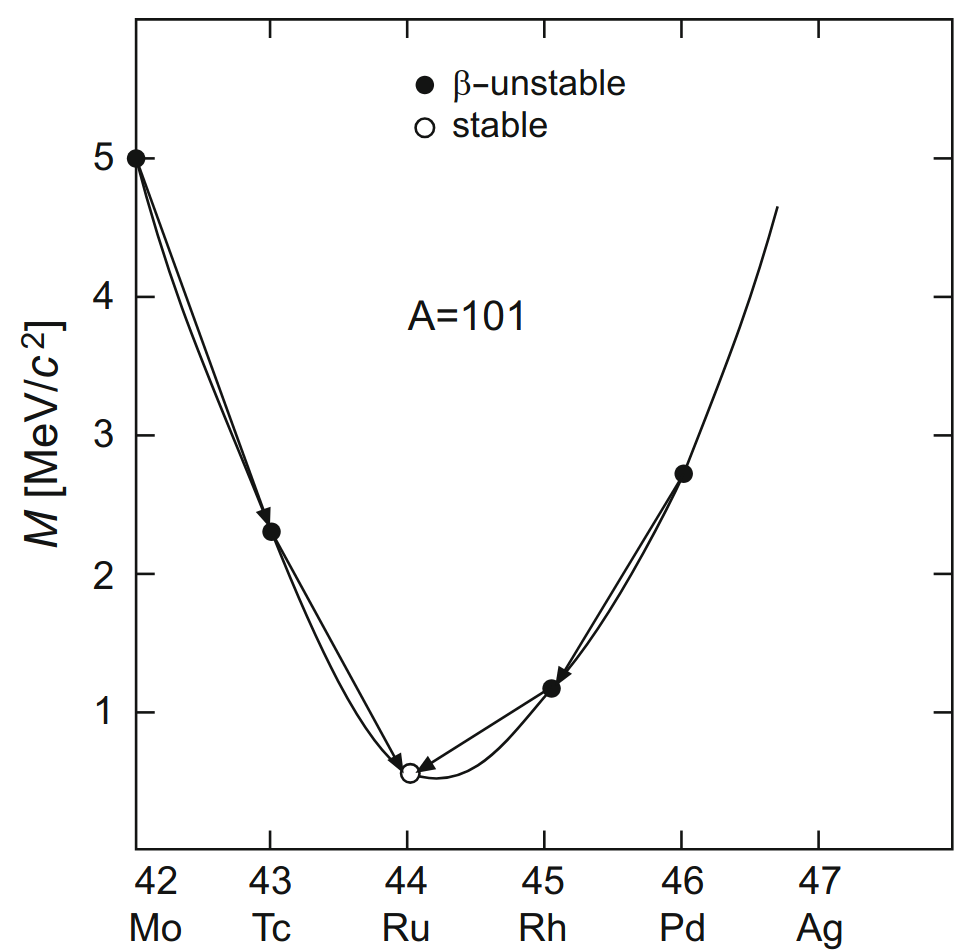
\includegraphics[width=0.60\textwidth]{iso-chain-odd.png}
	\caption{Isotopic chain with $ A = 101 $.}
	\label{iso-chain-odd}
\end{figure}
\begin{figure}
	\centering
	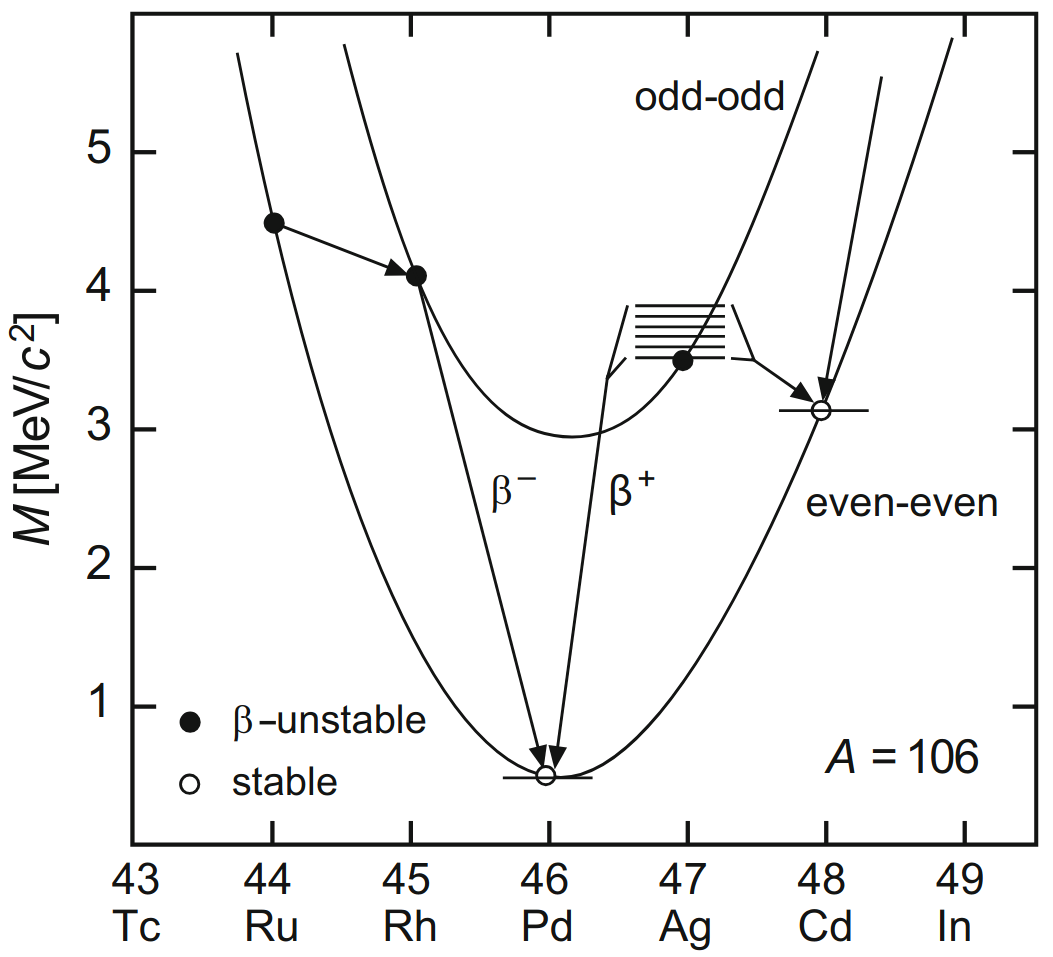
\includegraphics[width=0.60\textwidth]{iso-chain-even.png}
	\caption{Isotopic chain with $ A = 106 $.}
	\label{iso-chain-even}
\end{figure}

Tendenzialmente, i nuclidi instabili si riconducono alla stabilità tramite decadimento $ \beta $, sia $ p^+ \rightarrow n $ che $ n \rightarrow p^+ $. In casi particolari, alcuni nuclidi con $ N $ e $ Z $ dispari possono decadere con un doppio decadimento $ \beta $.\\
La formula semi-empirica ha un ottimo accordo coi dati sperimentali per i nuclei pesanti, con errori di circa $ \pm 1\% $, mentre per i nuclei leggeri sono presenti alcune discrepanze: a basso $ A $, il modello a goccia diventa poco accurato.\\
Inoltre, va notato che il modello presenta delle grosse incertezze (sia per le masse che per le abbondanze isotopiche) per isotopi senza valori sperimentali delle masse.

\subsection{Momento angolare e spin}











